\documentclass[tikz,border=2pt]{standalone}
\usepackage{amsmath,amssymb}
\usetikzlibrary{arrows.meta}

\begin{document}
% sgn along sequences: x_n -> 0+ (red) gives sgn(x_n) = 1, y_n -> 0- (green) gives sgn(y_n) = -1,
% so the one-sided limits at 0 are 1 and -1.
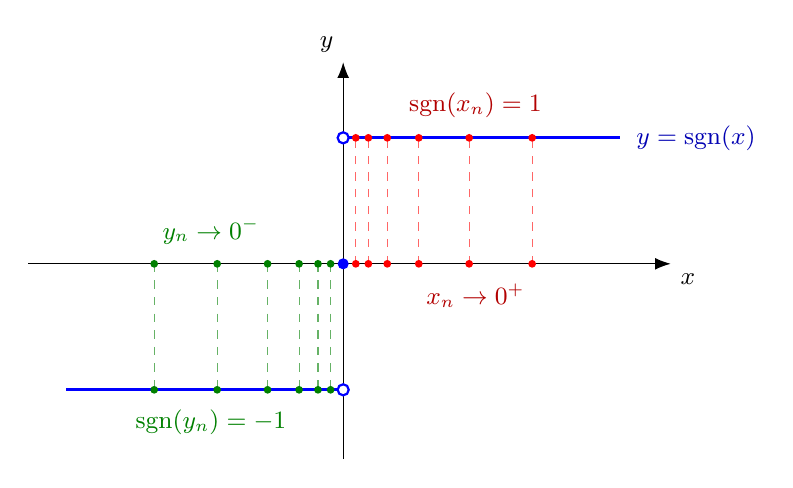
\begin{tikzpicture}[every node/.style={font=\small}, >={Latex[length=2mm]}, x=1.6cm, y=1.6cm]
	\draw[->] (-2.5,0) -- (2.6,0) node[below right] {$x$};
	\draw[->] (0,-1.55) -- (0,1.6) node[above left] {$y$};
	\draw[blue, very thick] (-2.2,-1) -- (-0.05,-1);
	\draw[blue, very thick] (0.05,1) -- (2.2,1);
	\draw[blue, thick, fill=white] (0,1) circle (2pt);
	\draw[blue, thick, fill=white] (0,-1) circle (2pt);
	\fill[blue] (0,0) circle (2pt);
	\foreach \t in {1.5,1,0.6,0.35,0.2,0.1} {
		\draw[red!60, dashed] (\t,0) -- (\t,1);
		\fill[red] (\t,0) circle (1.4pt);
		\fill[red] (\t,1) circle (1.4pt);
		\draw[green!50!black!60, dashed] (-\t,0) -- (-\t,-1);
		\fill[green!50!black] (-\t,0) circle (1.4pt);
		\fill[green!50!black] (-\t,-1) circle (1.4pt);
	}
	\node[red!70!black, anchor=north, font=\small] at (1.05,-0.08) {$x_n\to0^+$};
	\node[green!50!black, anchor=south, font=\small] at (-1.05,0.08) {$y_n\to0^-$};
	\node[red!70!black, anchor=south, font=\small] at (1.05,1.08) {$\mathrm{sgn}(x_n)=1$};
	\node[green!50!black, anchor=north, font=\small] at (-1.05,-1.08) {$\mathrm{sgn}(y_n)=-1$};
	\node[blue!70!black, anchor=west, font=\small] at (2.25,1) {$y=\mathrm{sgn}(x)$};
\end{tikzpicture}
\end{document}
